\section{Raum und Zeit}
\subsection{Raum}
Mechanik spielt im dreidimensionalen Raum. [affiner Raum] $\M{E}^3={\T(Menge aller Punkte im Raum)}$\\
Ein Punkt $P\in\M{E}^3$ wird durch Angabe eines Ortsvektors $\vec{r}\in\M{R}^3$ (dreidimensionaler Vektorraum) relativ zu einem Ursprung $O\in\M{E}^3$ Festgelegt: $\vec{OP}=\vec{P}$.
\begin{figure}[h]
\begin{center}
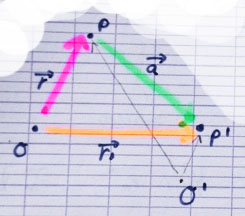
\includegraphics[width=0.4\textwidth]{Skizzen/Anhang13.jpg}
\end{center}
\caption{}
\end{figure}
Ein Skalarprodukt $\vec{r}\cdot\vec{r'}\in\M{R}^3$ liefert Längen\\
$\Rightarrow|\vec{r}|=\sqrt{\vec{r}\D\vec{r}}$\\
und abstände $d(P,P')=|\vec{a}|=|\vec{r}-\vec{r'}|=\sqrt{(\vec{r}-\vec{r'})\D\vec{r}-\vec{r'}}$
'Euklidischer' Raum $\M{E}^3$: affine, 3d Räume mit $d(P,P')$\\
\begin{description}
\item[Bemerkung]~\par
\begin{itemize}
\item Die Wahl von O ist beliebig, eine andere Wahl O' mag zweckmäßiger sein,'ändert nichts an der Physik' insbesondere gilt:$d_{O}(P,P')=d_{O'}(P,P')$
\item Übergang $O\rightarrow O'$: wechsel des Bezugssystems
\end{itemize}
\end{description}
\subsection{Koordinatensysteme}
für $P\in\M{E}^3$ muss angegeben werden: (Ursprung O) und (Koordinaten (x,y,z) bzgl. einer Karthesischen OB $e_1,e_2,e_3$ $e_i\D e_j=\delta_{ij}$\\
für den Punkt $P$ folgt dann:
\begin{align*}
\vec{OP}=\vec{r}=x\vec{e_1}+y\vec{e_2}+z\vec{e_3}=\sum_i^3 x_i\vec{e_i}
\end{align*}
den Punkt $P$ ordnen wir den Spaltenvektor $\vec{x}=\begin{pmatrix}
x \\ 
y \\ 
z
\end{pmatrix} $ zu bezogen auf $(O,\vec{e_1},\vec{e_2},\vec{e_3})$
\begin{description}
\item[Bemerkungen]~\par
\begin{enumerate}
\item Die Wahl von $(\vec{e_1},\vec{e_2},\vec{e_3})$ ist beliebig.\\
Es gilt: $(\vec{e_1},\vec{e_2},\vec{e_3})\rightarrow(\vec{e_1'},\vec{e_2'},\vec{e_3'})$\\
$\vec{e_k}=\sum_i R_{ki} \vec{e_i}$ mit einer orthogonalen Transformation $R\in O(3)$
Drehungsmatrix $R^{-1}=R^T; (\det R=1)$
\item Transformation der Koordinaten bezogen auf $(O,\vec{e_1},\vec{e_2},\vec{e_3})$
\end{enumerate}
\end{description}

\begin{description}
\item[Aktive Transformation]~\par
\begin{itemize}
\item die Rel. GL(") definiert bzgl eines festen Koordinaten- Systems (O,e,e,e) eine aktive Drehung R des Vektors $\vec{r}=\sum_k x_k\vec{e}_k \rightarrow \vec{r'}=\sum_k x'_k\vec{e_k}=R\vec{r}$
\end{itemize}
\begin{figure}[h]
\begin{center}
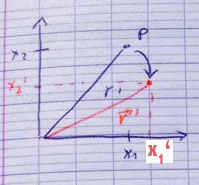
\includegraphics[width=0.4\textwidth]{Skizzen/Anhang11.jpg}
\end{center}
\caption{}
\end{figure}
\textbf{Achtung}:

für die Basisvektoren aus Bemerkung 2 gilt: $\vec{e_k'}=(R^{-1})\vec{e_k}$ siehe Vorübung
\item[Transformation] Die Trafo GL(") definiert allgemein das Transformations-verhalten eines Vektors (Tensor 1.Stufe)

Beispiele:\\
$\vec{v}=\frac{d\vec{r}}{dt} \rightarrow v_k'=\sum_iR_{ki}v_i$; Geschwindigkeit, Beschleunigung, etc.\\
Bedeutung: Physikalische Grundgleichungen müssen das Trafo Verhalten respektieren

Bsp: $m\ddot{\vec{r}}=\vec{F}$ in (O,e,e,e) $m\ddot{x_i}=F_i \rightarrow$ in (O,e',e',e') $m\ddot{x_i'}=F_i'$
\item[Krumliniges KO-System] in dem $x_i=x_i(q_1,q_2,q_3); i=1,2,3$ mag sinnvoll sein.

Beispiele: Zylinder $(r, \varphi, z)$ oder Kugelkoordinaten $(r, \Theta, \varphi)$\\
\textbf{Achtung!}: $\vec{e_i}\rightarrow\vec{e_i}(q_1,q_2,q_3)$
\end{description}
\newpage
\subsection{Zeit}
\subsubsection{Ereignis}
E ist ein Punkt der Raum-Zeit mit Koordinaten $(t,x,y,z)$ bezogen auf $(O,e,e,e)$
\begin{figure}[h]
\begin{center}
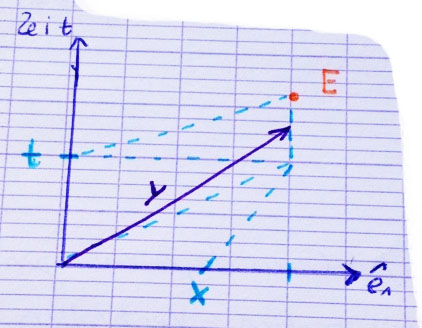
\includegraphics[width=0.4\textwidth]{Skizzen/Anhang10.jpg}
\end{center}
\caption{}
\end{figure}
\paragraph*{Ort}
räumliche Koordinaten $(x,y,z)$ werden abgelesen durch Maßstäbe.
\paragraph*{Zeit}
zeitliche Koordinate $t$ (Koordinatenzeit): abgelesen von einer Uhr\\
\begin{itemize}
\item Festlegung der Zeit $t$ eines Ereignisses gleichzeitiges betrachten von E und der Uhr
\item nur lokal möglich
\item wir denken uns im gesamten Raum ausgestattet mit Uhren, die alle synchronisiert sind.\\
\end{itemize}
Die Koordinatenzeit $t$ des Ereignisses E mit (t,x,y,z) wird von der Uhr mit räumlichen Koordinaten (x,y,z) abgelesen!

\subparagraph*{Bemerkung} 
\begin{enumerate}
\item die absolute Uhrzeit $t$ ist beliebig, eine andere Wahl $t'=t+t_0$ mag zweckmäßiger sein. 'ändert nichts an der Physik'
\item Uhrensynchronisation kann durch Lichtpulse realisiert werden ('Einstein-Synchronisation'), etwa vom Mittelpunkt zwischen zwei Uhren.\\
es zeigt sich: äquivalent dazu (sehr langsamer) Uhrentransport
\item Vorsicht ist geboten beim vergleich von Uhren in relativ zueinander bewegten Bezugssystemen
\end{enumerate}
\subsection{Kinematik}
Der klassischen Mechanik\\
Kin= 'Beschreibung der Bewegung' (ohne auf Ursachen einzugehen)
\begin{description}
\item[Bahnkurve] $\vec{r}(t)$
\item[Ortsvektor] 
\item[Geschwindigkeit] $\vec{v}(t)=\frac{d\vec{r}(t)}{dt}$\\
$\vec{v}(t)=\vec{v}(t)\D \vec{T}(t)$ mit $|\vec{T}|=1; v(t)=|\vec{v}(t)|$
\item[Beschleunigung] $\vec{a}(t)=\frac{d\vec{v}(t)}{dt}=\dot{t}\vec{T}+v(t)\dot{\vec{T}}(t)$

\begin{figure}[h]
\begin{center}
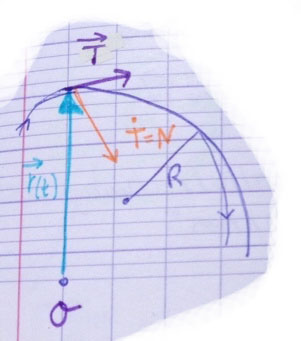
\includegraphics[width=0.4\textwidth]{Skizzen/Anhang9.jpg}
\end{center}
\caption{}
\end{figure}
\end{description}
$\vec{N}=\frac{\dot{\vec{T}}(t)}{|\dot{\vec{T}}(t)|}$ steht senkrecht auf $\vec{T}$ und $|\vec{N}|=1$ ('Normalenvektor')\\
$(T,N)$ definieren 'Schmiegeebene', in der lokal die Bahnkurve durch einen Kreis mit Kümmungsradius $R=\frac{v}{|\dot{\vec{T}}|}$ beschrieben werden kann (siehe Übung)\\
es folgt $\vec{a}=\dot{v}\vec{T}+\frac{v^2}{R}\vec{N}$\\
als summe von zwei orthogonalen Beiträgen wobei \\der erste: eine Tangentialbeschleunigung und \\der Zweite: eine Normal- oder Zentripetalbeschleunigung ist.
\newpage
\begin{description}
\item[Beispiel]~\par
\begin{enumerate}
\item geradlinig-gleichförmige Bewegung 
\begin{align*}
\vec{r}(t)=\vec{r_0}+\vec{v_0}t\\
\Rightarrow\vec{a}=0\\
(\dot{v}=0, R=\infty)
\end{align*}
\begin{figure}[h]
\begin{center}
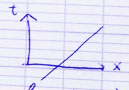
\includegraphics[width=0.4\textwidth]{Skizzen/Anhang8Kopie.jpg}
\end{center}
\caption{}
\end{figure}
\item geradlinig (allgemein)
\begin{align*}
\vec{r}(t)=\vec{r_0}+l(t)\vec{T_0}\\
\vec{v}=\dot{l}\vec{T_0} \\
v=\dot{l} \\
\vec{T}=\vec{T_0} \\
(\dot{v}=\ddot{l}; R=\infty)
\end{align*}
\begin{figure}[h]
\begin{center}
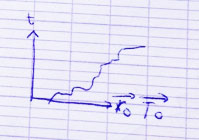
\includegraphics[width=0.4\textwidth]{Skizzen/Anhang8.jpg}
\end{center}
\caption{}
\end{figure}
\item gleichförmige Kreisbewegung
\begin{align*}
v=const.=\frac{2\pi R}{\tau}\\
\dot{v}=0\\
\vec{a}=\frac{v^2}{R}\D \vec{N}=4\pi^2\frac{R}{\tau^2}\vec{N}
\end{align*}
$\tau$ Umlaufzeit\\
Anwendung auf Kepler-Bahnen für Planeten $\tau^2\sim R^3$ (3.Keplergesetz)\\
$\Rightarrow\vec{a}\sim \frac{1}{R^2}\vec{N}$ ($\vec{F}=m\vec{a}) \Rightarrow$ Planetenbewegung $\vec{F}\sim \frac{1}{R^2}\vec{N}$
\begin{figure}[h]
\begin{center}
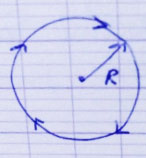
\includegraphics[width=0.4\textwidth]{Skizzen/Anhang7.jpg}
\end{center}
\caption{}
\end{figure}
\end{enumerate}
\end{description}
\subsection{Bewegte Bezugssysteme und Inertialsysteme}
RS=Ruhesystem\\
Wie wählen wir (o,e,e,e) \underline{geeignet}?\\
\begin{itemize}
\item nahe liegend \underline{Laborsystem} (Labortisch ruht im LS)\\
\underline{Beispiel} elastischer Stoß im LS (m ruht)
\end{itemize}
\begin{figure}[h]
\begin{center}
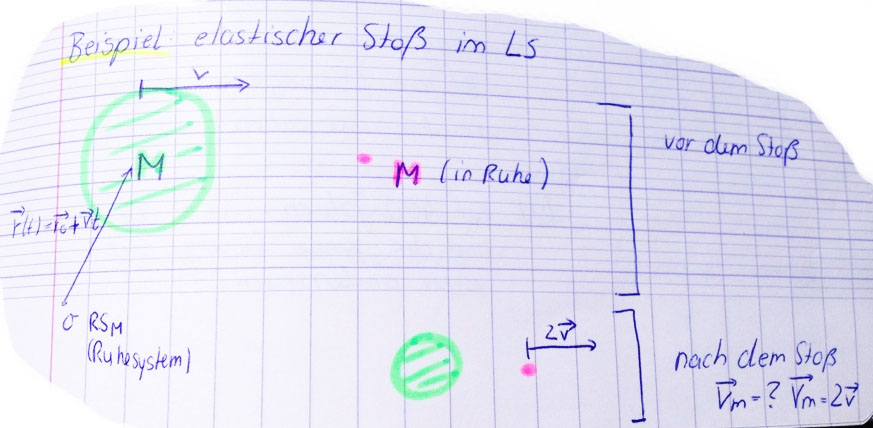
\includegraphics[width=0.4\textwidth]{Skizzen/Anhang6.jpg}
\end{center}
\caption{}
\end{figure}
\newpage
wechsle ins Ruhesystem der Masse M\\
die betrachtung wird eindeutig und trivial bei $M\gg m$\\
Übergang von System Labortisch (O,e,e,e, Uhren) in RS der großen Masse M (O',e',e',e',Uhren') gilt:
\begin{align*}
\vec{r'}=\vec{r}-\vec{v}t\\
t'=t
\end{align*}
\begin{figure}[h]
\begin{center}
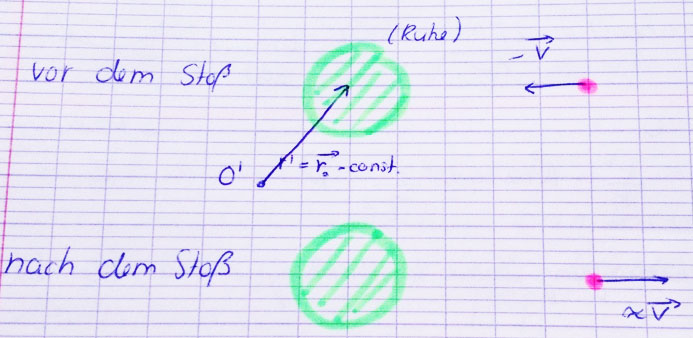
\includegraphics[width=0.4\textwidth]{Skizzen/Anhang5.jpg}
\end{center}
\caption{}
\end{figure}

Die \textbf{Galilei-Transformation} beschreibt Transformationsgesetz von BS zu BS', das sich mit Geschwindigkeit $v$ relativ zu BS bewegt. Zur Beschreibung sind $BS=RS_m$ und $BS'=RS_M$ völlig gleichwertig (hier $BS'$ transparenter).\\
\subparagraph*{Bemerkungen}
\begin{enumerate}
\item Zustand \textbf{'in Ruhe'} hat keine Absolute Bedeutung sonder hängt von der Wahl des Bezugssystems ab. (Bewegung ist \underline{relativ} zu sehen)
\item vor 400Jahren: ruht die Erde und die Sonne bewegt sich?\\
Galilei: Frage ist bedeutungslos, nicht entscheidbar\\
$\Rightarrow$ Galilei-Transformationen
\item Relativität kommt zum Ausdruck im 1. Newtonschen Gesetz:('Trägheitssatz')\\
Ein Körper verharrt im Zustand der Ruhe oder der geradlinig-gleichförmigen Bewegung sofern er nicht durch Kräfte zur Änderung gezwungen wird.
\end{enumerate}
\subsubsection{Inertialsysteme}
(IS) sind BS, die durch die Gültigkeit des 1. Newtonschen Gesetzes ausgezeichnet sind. Ausgehend von einem IS findet man weitere IS' durch geradlinig-gleichförmige Bewegung des IS' relativ zu IS.(häufig IS='ruhend bzgl. des Fixsternhimmels'; in der Praxis LS$\approx$IS (gute Näherung)).\\
in einem relativ zu IS \underline{beschleunigten} BS treten \underline{Scheinkräfte} auf, die nicht auf fundamentalen Wechselwirkungen (Coulombkraft, etc) beruhen.\\
$\Rightarrow$ physikalische Grundgesetze werden bzgl. eines IS formuliert, dabei sind \underline{alle} IS völlig gleichwertig; IS$\rightarrow$IS' durch:
\begin{enumerate}
\item 'boost' mit Richtung $\vec{v}$ $t'=r(t-\frac{\vec{v}\vec{r}}{c^2})$
\item gleichförmig-geradlinige Bew: $\vec{r'}=\vec{r}-\vec{v}t$ (3 Parameter)\\
(Galilei-Relativität)
\item räumliche Verschiebung: $\vec{r'}=\vec{r}+\vec{r_0}$ (3 Parameter)\\
(Homogenität des Raumes)
\item räumliche Drehung: $\vec{r'}=R\vec{r}$ (3 Parameter)\\
(Isotropie des Raumes)
\item zeitleiche Verschiebung: $t'=t+t_0$ (1 Parameter)\\
(Homogenität der Zeit)
\end{enumerate}
Die Kombination all dieser Transformationen definieren die \emph{'Galilei-Gruppe'} der klassischen Raum-Zeit mit 10 freien Parametern.
\subsection{Galilei- und Lorenztransformationen}
Die Naturgesetze müssen von einer Art sein, die (form-)invariant sind unter Transformation zwischen IS\\
Bsp.: IS$\rightarrow$IS', dann:\\
Newton:
\begin{align*}
m\frac{d^2 \vec{r}}{dt^{2}}=\vec{F} \Leftrightarrow m\frac{d^{2}\vec{r'}}{dt'^{2}}=\vec{F'}
\end{align*}
$\rightarrow$ \emph{Relativitätsprinzip!} insbesondere gilt:\\
geradlinig-gleichförmige Bewegung in IS mit Koordinaten(t,x,y,z) ist auch eine
geradlinig-gleichförmige Bewegung in einem anderen IS' mit (t',x',y',z').
\\
\begin{description}
\item[Bsp: Galilei-Transformaiton]: mit $\vec{v}$ rel. zu IS bew. IS' gilt $\vec{r'}=\vec{r}-\vec{v}t$, $t'=t+t_0$\\
in IS: $\vec{r}(t)=\vec{r_0}+\vec{u}t$\\
$\Rightarrow IS': \vec{r'}(t')=\vec{r_0}+(\vec{u}-\vec{v})t'$\\
\item[Umkehrung?] folgt aus der Forderung (s.o.) dass $t,\vec{r}\rightarrow t',\vec{r'}$ eine Galilei-Trafo?\\
Frage: 'wie sieht allgemein eine Trafo $(t,x,y,z)\rightarrow(t',x',y',z')$ aus, die die Forderung (s.o.) erfüllt f+r IS$\rightarrow$IS', das sich mit $\vec{v}$(vorgegeben) relativ zu IS bewegt?
\begin{figure}[h]
\begin{center}
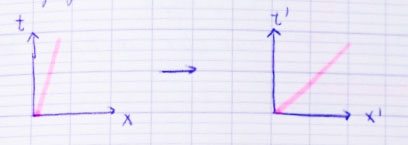
\includegraphics[width=0.4\textwidth]{Skizzen/Anhang4.jpg}
\end{center}
\caption{}
\end{figure}
\begin{itemize}
\item lineare Trafo der Raum-Zeit! $\begin{pmatrix}
t'\\
x'\\
y'\\
z'
\end{pmatrix}
=\begin{pmatrix}
. & . & . & . \\
.\\
. & 4 & \times & 4\\
.
\end{pmatrix}
\begin{pmatrix}
t\\
x\\
y\\
z
\end{pmatrix}
$
\item bzgl. räumlicher Anteile $\vec{r}$ Vektorcharakter muss erhalten bleiben: $\vec{r'}\sim\vec{r},\vec{v}$
\item Ansatz:
\begin{align*}
t'=a	(v)			t+b(v) 			(\vec{v}\D \vec{r})\\
\vec{r'}=c(v)		\vec{r}+\frac{d(v)}{v^2}	(\vec{v}\D\vec{r})\vec{v}+e(v)		\vec{v}t
\end{align*}
mit beliebigen Funktionen $a(v),...,e(v)$, die bestimmen weitere Forderungen:
\end{itemize}
\begin{enumerate}
\item für $\vec{r}=\vec{v}t \Rightarrow \vec{r'}=0 \Rightarrow c+d+e=0$
\item Relativität (I) Vertausche Rolle IS$\leftrightarrow$IS' ($\vec{v}\rightarrow-\vec{v}$)\\
\begin{align*}
\Rightarrow t=a(v)t'-b(v)(\vec{v}\vec{r'})\\
\vec{r}=c(v)\vec{r'}+\frac{d(v)}{v^2}(\vec{v}\D\vec{r'})\vec{v}+e(v)\vec{v}t'
\end{align*}
ersetze $t'$ und $\vec{r'}$ auf der rechten Seite durch Ansatz\\
\begin{align*}\Rightarrow t=a(v)(a(v)t+b(v)(\vec{v}\vec{r})-...\\
\vec{r}=c(v)(c(v)\vec{r}+...)+...\vec{v}...\\
\Rightarrow c^2=1; a=c+d; a^2=1+ebv^2; e=-a\\
\Rightarrow c=1; e=-a; d=a-1; b=\frac{1-a^2}{av^2}
\end{align*}
Wähle Koordinatensystem so, dass x in Richtung $\vec{v}$ zeigt.
$\Rightarrow \vec{v}=\begin{pmatrix}
v\\
0\\
0
\end{pmatrix}$
\begin{align*}
t'=a(v)t+\frac{1-a^2(v)}{a(v)v}x\\
x'=a(v)(x-vt); y'=y; z'=z
\end{align*}
\item Relativitätsprinzip:\\
IS$\rightarrow^v$ IS'$\rightarrow^u$ IS''\\
\begin{align*}
t'' &=a(u)t'+\frac{1-a^2(u)}{a(u)u}x'=a(u)(a(v)t+\frac{1-a^2(v)}{a(v)v}x)+\frac{1-a^2(u)}{a(u)u}(a(v)(x-vt))\\
x'' &=a(u)(x'-ut')=a(u)(a(v)-u\frac{1-a^2(v)}{a(v)v})x+...t
\end{align*}
außerdem muss gelten IS$\rightarrow^w$ IS''\\
woraus folgt, dass
\begin{align*}
t''=a(w)t+(w)x\\
x''=a(w)(x-wt)
\end{align*}
woraus dann folgt:
\begin{align*}
[a(u)a(v)-\frac{va(v)}{ua(u)}			&(1-a^2(u)]t+...x \\
a(u)a(v)-\frac{va(v)}{ua(u)}(1-a^2(u) 	&=a(w)\\
\Rightarrow\frac{a^2(u)-1}{u^2a^2(u)} 	&=\frac{a^2(v)-1}{v^2a^2(v)}\\
\Rightarrow \frac{a^2(v)-1}{v^2a^2(v)} 	&=const.=K \\
\Rightarrow a(v) 						&=\frac{1}{\sqrt{1-Kv^2}}\\
 k=0\Rightarrow a=1 						&\Rightarrow \text{ist Galilei Trafo}\\
 k\neq 0? [k]=\frac{1}{\text{Geschwindigkeit}^2} &=\frac{1}{c^2}=const.
\end{align*}

\begin{align*}
 \Rightarrow &t'=a(v)(t-\frac{vx}{c^2})\\
 &x'=a(v)(x-vt)
\end{align*}
Die Lorentz-Transformation mit $a(v)\rightarrow \gamma(v)=\frac{1}{\sqrt{1-\frac{v^2}{c^2}}}$\\
Bedeutung von $c$?\\
Man betrachte die 'Addition' von Geschwindigkeiten: $w=u+v$?
\begin{align*}
a(w)		&=a(v)a(u)(1+kuv)\\
1-kw^2	&=\frac{(1-kv^2)(1-ku^2)+(1+kuv)^2-(1+kuv)^2}{(1+kuv)^2}\\
		&=1-k\frac{(u+v)^2}{(1+kuv)^2}\\
\Rightarrow w	&=\frac{u+v}{1+kuv}\Leftrightarrow(\frac{w}{c})^2\\
		&=\frac{(\frac{u}{c}+\frac{v}{c})^2}{(1+\frac{uv}{c^2})^2}\\
		&=1-\frac{(1-\frac{u}{c}^2)(1-\frac{v}{c}^2)}{(1+\frac{u}{c}\frac{v}{c})^2}
\end{align*}
\underline{Folgerungen}:
\begin{enumerate}
\item für $u=c\Rightarrow w=c$
\item für $v=c\Rightarrow w=c$
\item für $u<c; v<c \Rightarrow w<c$
\item für $u\ll c; v\ll v \Rightarrow w\approx u+v$
\end{enumerate}
$c$ ist Lichtgeschwindigkeit
\end{enumerate}
\subparagraph*{Raum-Zeit-Diagramme}
\begin{figure}[h]
\begin{center}
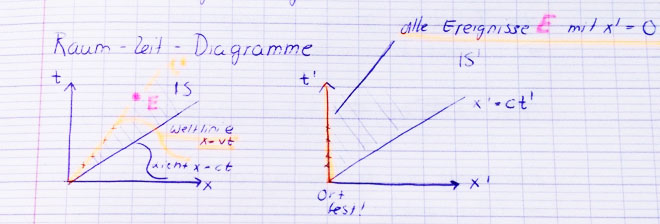
\includegraphics[width=0.4\textwidth]{Skizzen/Anhang3Kopie.jpg}
\end{center}
\caption{}
\end{figure}
\end{description}